\chapter{Implementácia}\label{impl}
Implementácia začala komunikáciou s~firmou \emph{Logimic} opísanou v~kapitole \ref{Logimic}. Tá mi poskytla senzory \emph{RisingHF1S001} s~proprietárnou \emph{TTI bránou} firmy \emph{The Things Industries\footnote{Viac o~firme na stránkach \url{https://www.thethingsindustries.com}.}}. 
Obe zariadenia sú pre LoRaWAN riešenia. 
Implementácia sa teda ďalej, ako podľa plánu, sústredí na túto technológiu. 
Nanešťastie v~priebehu implementácie sa firma \emph{Logimic} rozhodla ukončiť spoluprácu s~\emph{The Things Industries} a musel som svoju prácu migrovať inam a teda začínať nanovo. 
Táto kapitola ďalej pokračuje od tohto momentu a prechádza implementáciou na základe hlavných komponentov architektúry z~kapitoly \ref{navrh-architektura}. 
Teda podkapitola \ref{impl-IOT} sa venuje všetkým využitým \emph{IoT} zariadeniam, ich inštalácii a konfigurácii. 
Podkapitola \ref{impl-Chirp} sa venuje LoRaWAN sieťovému serveru (ďalej využívana skratka LNS), na ktorom sú zariadenia zaregistrované. Ďalej sa venuje kóderu a dekóderu, ktoré na ňom pracujú. 
Následne, podkapitola \ref{impl-Lambda} sa venuje cyklickej službe. Nakoniec podkapitola \ref{impl-iTemp} vysvetľuje postup prípravy užívateľskej aplikácie \emph{iTemp} na toto riešenie.

Celá implementácia je vytvorená v~integrácii s~riešením \emph{iTemp}. To znamená, že nie je presne podľa návrhov z~kapitoli \ref{navrh}. 
Napriek tomu je návrh stále podobný implementácii. Všetky konfiguračné súbory, kódy a programy vytvorené pre túto bakalársku prácu sú dostupné na \emph{GitHub}\footnote{Konkrétny link je \url{https://github.com/Siki-ux/bp-int-heating}.}.


\section{IoT zariadenia}\label{impl-IOT}
Následujúce podkapitoly sa venujú konkrétnym zariadeniam použitých pri implementácii. Všetky zariadenia boli poskytnuté firmou \emph{Logimic}.
\subsection{RisingHF1S001}\label{impl-Rising}
Je to \emph{LoRaWAN} bezdrátový senzor teploty a vlhkosti vyrábaný firmou \emph{RisingHF\footnote{Viac o~firme na stránkach \url{https://www.risinghf.com/home}.}}. 
Toto kompaktné zariadenie pracujúce na batériach môže byť inštalované v~rôznych podmienkach na rôznych miestach. 
V~tomto prípade bude slúžiť hlavne ako teplotný senzor umiestnený v~miestnosti na mieste, kde chce užívateľ dosiahnuť požadovanú teplotu.
\subsection*{Inštalácia}
Inštalácia tohto zariadenia je jednoduchá a spočíva iba v~uvoľnení šrúb vonkajšieho obalu a zapojení batérie.
\subsection*{Konfigurácia}
Konfigurácia vyžaduje proprietárny konfiguračný nástroj \emph{RCFG Tool} firmy \emph{RisingHF}. Zariadenie zbavené vonkajšieho obalu pripojíme USB-mini B káblom k~počítaču. Následne spustíme konfiguračný nástroj. Ním môžme nahrať do zariadenia konfiguračný súbor. Mimo iné je v~ňom najdôležitejšie nakonfigurovať komunikačné kanály, kľúč aplikácie (\emph{AppKey}) pre aktiváciu vzduchom (\emph{OTAA}) a zabezpečenie komunikácie. 

\subsection{MClimate Vicki LoRaWAN}\label{impl-Vicki}
Toto zariadenie je bližšie opísané v~kapitole \ref{analyza-solutions} v~části o~technológii \emph{LoRaWAN}. Pri začiatku implementácie vyšlo toto zariadenie ako najvýhodnejšie.
\subsection*{Inštalácia}
Najskôr je potrebné odpojiť zadný kryt hlavice. 
Ten následne pripojiť na termostatický ventil. Do samotnej hlavice následne zapojiť batérie. Počkať na svetelnú signalizáciu hlavice a~následne ju pripojiť k~zadnému  krytu na termostatickom ventile. Zariadenie následne prejde do kalibračného režimu na niekoľko minút. Po zobrazení nastavenej teploty na displeji je kalibrácia hotová a zariadenie je pripravené na prácu.
\subsection*{Konfigurácia}
Zariadenie prichádza predkonfigurované s~konfiguráciou zameranou na aplikáciu \emph{MClimate Enterprise\footnote{Viac informácii na \url{https://mclimate.eu/pages/enterprise}.}}. Z~tejto aplikácie je možné prenastaviť predvolený \emph{LoRaWAN} server na server \emph{Chirpstack}, ktorý je opísaný v~nasledujúcej podkapitole \ref{impl-Chirp}.


\subsection{Mikrotik wAP LR8}
Jedná sa o~bedrátový prístupový bod (\emph{AP}) produkovaný firmov \emph{Mikrotik\footnote{Viac informácii o~firme na \url{https://mikrotik.com}.}}. Má množstvo funkcii\footnote{Zoznam dostupný na \url{https://mikrotik.com/product/wap_lr8_kit}.}, no pre riešenie tejto práce sú relevantné najmä: možnosť prijímať LoRaWAN komunikáciu a možnosť použiť ho ako most medzi \emph{Chirpstack} serverom, opísanom v~podkapitole \ref{impl-Chirp} a \emph{IoT zariadeniami}, opísaných v~podkapitole \ref{impl-IOT}.
\subsection*{Inštalácia}
Spodný kryt zariadenia je zabezpečený jednou skrutkou. 
Po jej odšrubovaní sa ukáže priestor na pripojenie zdroja energie, ethernetový port a port antény. 
Následne sa pripojí anténa a ako zdroj energie použijeme technológiu \emph{PoE} (Power over ethernet), teda zdroj energie pôjde pripojeným ethernetovým káblom. Následne zasunieme zadný kryt a~zaistíme ho skrutkou.
\subsection*{Konfigurácia}
Zariadenie funguje ako prístupový bod. Vďaka tomu sa na neho dá pripojiť technológiou \emph{Wi-fi} a prístupom na adresu \emph{192.168.88.1}. 
Tak sa dá dostať do ovládacieho rozhrania zariadenia. V~sekcii \emph{LoRa} vytvoríme pripojenie na LNS a zapneme službu tejto brány. 
V~tomto momente začne zariadenie prijímať LoRa správy a bude ich ďalej posúvať na LNS.  


\section{Registrácia zariadení}\label{impl-Chirp}
 Zariadenia je potrebné registrovať na LoRaWAN sieťový server.
 K tomu bol zvolený Chirpstack.
 Ten je open-source LoRaWAN sieťový server a aplikačný server, ktorý poskytuje kompletné riešenie na budovanie, nasadzovanie a spravovanie LoRaWAN sietí. 
 S~jeho využitím je možné jednoducho vytvárať vlastné aplikácie pre monitorovanie, riadenie a správu LoRaWAN zariadení a senzorových dát.
 ChirpStack umožňuje aj vytvorenie rozšíriteľných IoT riešení a ich integráciu do existujúcich systémov a cloudových platform, teda riešenia firmy \emph{Logimic}. 
 Podstatnou časťou platformy Chirpstack je preklad surových neformátovaných dát na dáta zrozumiteľné pre cloudové riešenie \emph{iTemp}. 
 K~tomu sa využívajú dva programy spoločne označované ako \emph{Codec}, patriace konkrétnym typom zariadení. Sú to kóder a dekóder, ktoré sú opísané ďalej.
\subsection*{Kóder}
Jedná sa o~program, ktorý sa spustí nad príchodzími datami z~aplikácie a vytvára preklad do formy pochopiteľnej pre zariadenie, ktoré týmto príkazom bude ovládať. V~tomto riešení sú vstupné dáta vo formáte JSON a výstupom je správa vo formáte \emph{Base64}. Chirpstack preklad do \emph{Base64} vytvára sám a požaduje k~tomu aby výstup kódera bol reťazec v~číselach desiatkovej sústavy o~veľkosti jedného bajtu.

To sa dá dosiahnúť postupným rozoberaním vstupnej JSON správy. Kde sa  podľa návrhu očakáva, že pod kľúčom \texttt{cmdName} sa nachádza názov príkazu, ktorý sa má vykonať. 
Prepínačom sa rozdelí do konkrétnej obsluhy daného príkazu, kde ďalej očakáva že pod kľučom \texttt{cmdPars} budú jednotlivé parametry daného príkazu. Následne sa do reťazca postupne pridá kód daného príkazu a vyformátované parametre. Prípadne je vykonaná kontrola vstupných parametrov, kde je možné, že by nesprávna hodnota mohla poškodiť zariadenie.

\subsection*{Dekóder}
Jedná sa o~program, ktorý sa spustí nad prichádzajúcimi datami od zariadení a vytvára preklad do formy pochopiteľnej pre aplikáciu a databázu. Dekóder dostáva vstupné dáta ako čísla v~desiatkovej sústave o~veľkosti jedného bajtu v~reťazci. Výstupom je zas správa vo formáte JSON v~štruktúre vytvorenej a vyžadovanej aplikáciou opísanou v~podkapitole \ref{impl-iTemp}.

To sa dá dosiahnuť dešifrovaním prvého čísla reťazca na jednotlivé parametre na základe implementácie zariadenia výrobcom. Ďalej podľa parametru nasledujúci určitý počet čísel v~reťazci patrí danému parametru a reprezentuje jeho hodnotu. Ak sa ďalej nachádzajú ďalšie čísla znamená to, že následuje ďalší parameter a proces sa opakuje. Tieto parametre sa postupne zapisujú pod kľúč \texttt{devPars} pod ich vlastým kľúčom.

\section{Obsluha zariadení}\label{impl-Lambda}
Jedná sa o~cyklickú službu \emph{AWS Lambda\footnote{Viac informácii o~službe na \url{https://aws.amazon.com/lambda/}.}}, ktorá spúšťa určité funkcie ako reakciu na napríklad prichádzajúce data alebo ich spúšťa v~určitom časovom intervale. V~tomto riešení je funkcia \texttt{HeatingControl} volaná v~intervale 5 minút. To z~dôvodu potreby zariadenia spraviť dva cykly správ \emph{keep-alive}. \emph{Keep-alive} je správa, ktorú hlavica posiela periodicky v~intervale 2 minút. Správa obsahuje potrebné informácie na výpočty funkcie \texttt{HeatingControl}. Dôvod potreby dvoch cyklov spočíva v~tom, že prvá správa potvrdí príjem zaslaného príkazu a druhá zašle aktuálne dáta na databázu.

Funkcia \texttt{HeatingControl} sa pred zavolaním pripojí do databázy \texttt{iTemp2}, čo je ostrá databáza riešenia \emph{iTemp}. 
Po úspešnom naviazaní spojenia si funkcia získa všetky hlavice, ktoré má ovládať.
Ako ukazuje diagram na obrázku \ref{fig:diagram}, dosiahne to prístupom do databázy funkciou \texttt{getDeviceList} s identifikačným číslom (ďalej používaná skratka ID) modelu hlavice, ktorá následne vráti list hlavíc.  
Z neho je pre každú hlavicu získané konkrétne ID systému, v ktorom sa hlavica nachádza a ID konkrétnej hlavice.
Každá hlavica sa nachádza v nejakej skupine, ktorá reprezentuje miestnosť, v ktorej je nainštalovaná. Preto je potrebné získať skupiny, v ktorých sa nachádza ďalším prístupom do databázy. 
To funkciou \texttt{getGroupList} s parametrom ID systému a ID hlavice, ktorá vráti list skupín tohto systému, v ktorých je hlavica nainštalovaná. Následne je možné pre každú ovládanú miestnosť získať z databázy konkrétne hodnoty parametrov ovládanej miestnosti. 
To funkciou \texttt{getDeviceParameterValueList} s parametrom ID hlavice, ktorá vráti list obsahujúci všetky parametry danej hlavice. 
Skupina, teda miestnosť môže používať externé teplotné senzory. K tomu je použitá funkcia \texttt{getRoomTemp}, ktorá v prípade že nájde v miestnosti teplotné senzory, vypočíta z ich nameraných teplôt priemer. 
Ak miestnosť nepoužíva teplotné senzory vráti hodnotu nameranú na hlavici.

Na základe získaných parametrov funkcia \texttt{HeatingControlLogic} začne vyhodnocovať situáciu. To spôsobom opísaným v podkapitole \ref{navrh-algo}. Teda najprv skontroluje, či je vôbec nutné spúšťať výpočet na základe rozdielu nameranej a cieľovej teploty. 
Ak je rozdiel dostatočný zistí, či je potrebné miestnosť vyhriať alebo  
naopak ochladiť. 
Ďalej sa skontroluje, či sa teplota od minulého cyklu pohla požadovaným smerom. Ak áno, nieje potrebné upraviť pozíciu motora. Ak nie, je potrebné prepočítať otvorenie motora na hlavici. 
Tento výpočet zabezpečuje funkcia \texttt{HeatingAlgo} volaná s parametrami miestnosti. 
Tá vypočítava pozíciu motora na základe vzorca \ref{eq:MPcalculation}. 
K tomu kontroluje, či je výsledok výpočtu a pôvodné nastavenie rozdielne o minimálny rozdiel krokov motora určeného v podkapitole \ref{navrh-algo}. 
Ak nie je, funkcia vráti pôvodné nastavenie. 
V prípade, že je výsledok mimo hranice motora, funkcia vráti najbližšiu hranicu. 
Funkcia \texttt{HeatingControlLogic} po získaní pozície motora vráti list s potrebnými datami. 
Z tohto listu sa ešte raz získa pozícia motora, ktorá sa porovná s predošlou pozíciou motora. 
V prípade, že nie sú rovnaké vyšle sa príkaz funkciou databázy \texttt{putLaunchCmdDevice} s parametrami ID hlavice, ID požadovaného príkazu a listom získaným z funkcie \texttt{HeatingControlLogic}. Následne je už len potrebné aktualizovať data v databáze. To funkciou \texttt{updateLastValue}, ktorá pripraví data do databázy a funkciou databázy \texttt{putDeviceParameterValueList} aktualizuje naposledy nameranú teplotu na momentálne nameranú teplotu.

 Funkcia \texttt{HeatingContorlLogic} je volaná nad každou hlavicou.
 Funkcia \texttt{HeatingControl} nakoniec vráti status 0, znamenajúci úspešné ukončenie ovládania.

\begin{figure}[H]
    \centering
    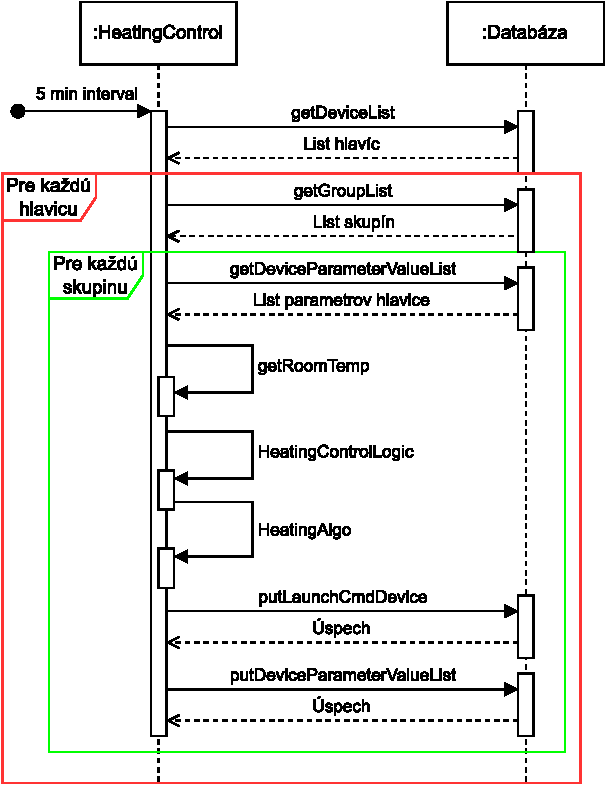
\includegraphics[width=0.8\textwidth]{obrazky-figures/diagram.pdf}
    \caption{Diagram služby ovládania kúrenia.}
    \label{fig:diagram}
\end{figure}

\section{Užívateľská aplikácia}\label{impl-iTemp}
Tou sa stala aplikácia iTemp.
Tá predstavuje bezdrôtové riešenie monitoringu vnútorného a vonkajšieho prostredia najmä teploty a vlhkosti.
Pracuje s~mnohými typmi senzorov ako je IQAROS sada\footnote{Viac informácii na \url{https://iqaros.cz/custom.html}}, LoRa teplotné senzory a ďalšie. 
Informácie máte v~telefóne, tablete, alebo domácom touch screene. Systém nielen monitoruje ale tiež informuje o~prekročených hodnotách a ukladá dlhodobo štatistiky.

V~rámci tohto riešenia je potrebné využitie \emph{SQL nástroja}  v~module administrácie. 
Tu sa vytvárajú typy parametrov, parametre a ich napríklad jednotky, ktoré sa skladajú do do modelov zariadení. Model zariadenia Vicki je možné vidieť na obrázku \ref{fig:model}.
Takýmto spôsobom sa pripraví databáza pre zariadenie a zadefinujú konktrétne kľúče \emph{JSON} správ. 
Následne je potrebné vytvoriť modely príkazov, ktoré budú posielané na zariadenie. 
Skladajú sa z~parametrov, ktoré budú upravovať a vytváraju tak \emph{JSON} správu, ktorej \emph{kóder} z~podkapitoli \ref{impl-Chirp} rozumie a po preložení ju zašle na zariadenie. 
Príkazy je potrebné ďalej priradiť konkrétnym zariadeniam.

Po príprave databázy, následuje založenie skupín, teda pre toto riešenie miestností, ktoré chceme ovládať zariadeniami. 
To sa vykonáva tak isto v~administrátorskom module. 
V~tomto konkrétnom riešení je ovládaná jedna miestnosť s~jedným regulátorom a dvoma tepelnými senzormi. 
Voliteľne je možné si nastaviť \emph{KPI} skupiny pre lepší prehľad z~domovskej obrazovky. V~tomto momente je regulácia teploty v~miestnosti ovládaná obsluhov z~predchádzajucej  kapitoly \ref{impl-Lambda}.

Pre zobrazenie konkrétnych dát, štatistík, grafov a zaslaných príkazov je potrebné prejsť cez skupinu na konkrétne zariadenie.

\begin{figure}[H]
    \centering
    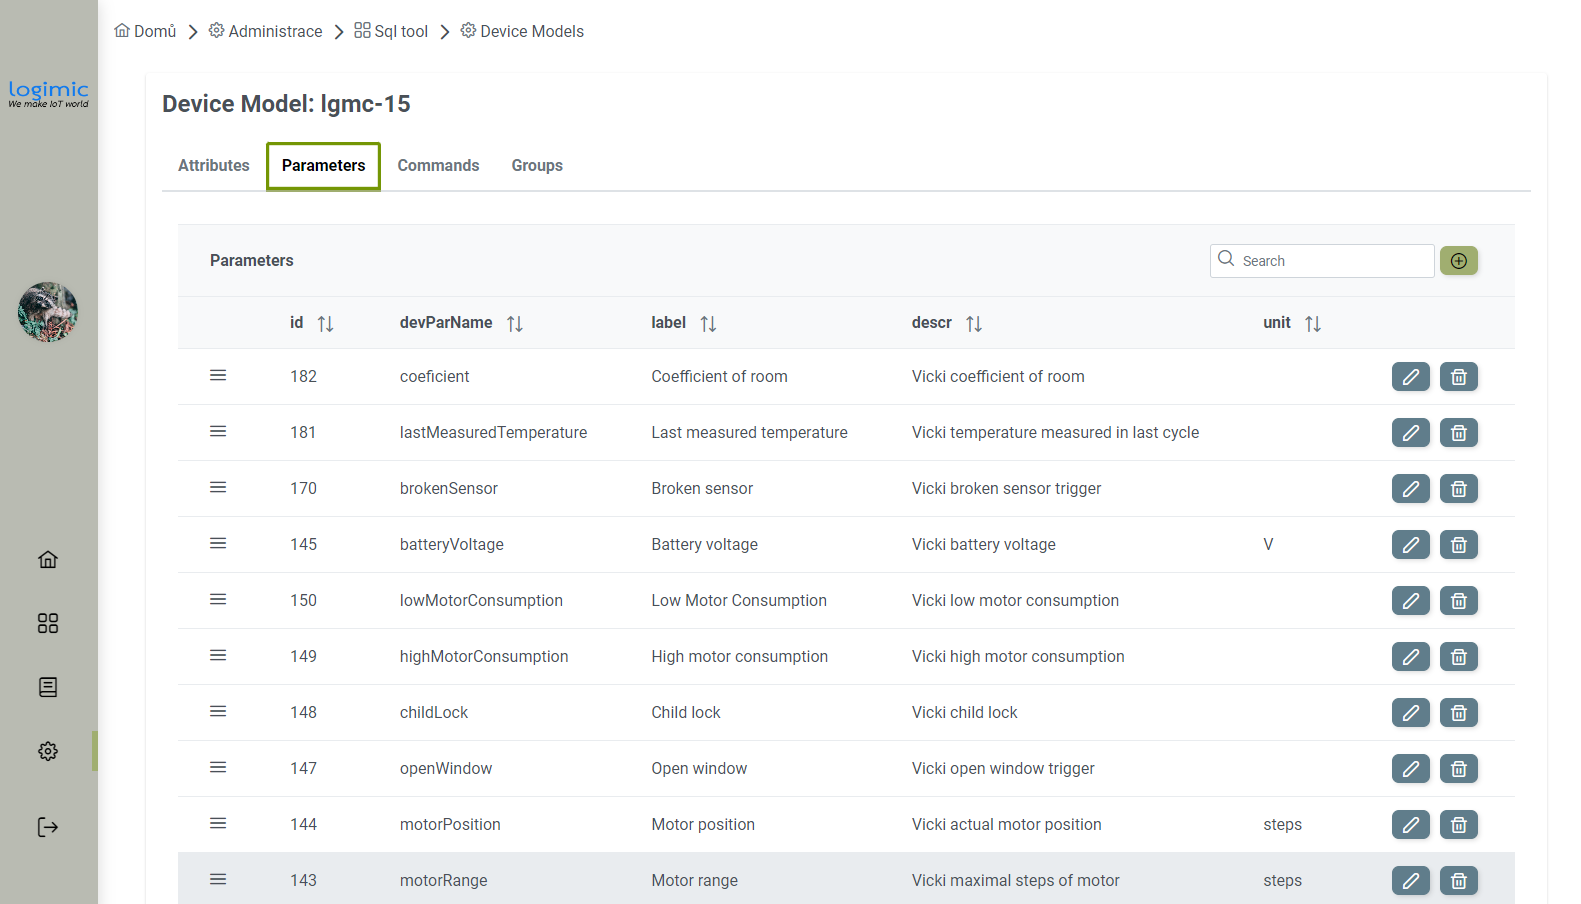
\includegraphics[width=\columnwidth]{obrazky-figures/Screenshot_13.png}
    \caption{Model zariadenia Vicki v SQL nástroji aplikácie iTemp.}
    \label{fig:model}
\end{figure}